\renewcommand{\thesection}{\Roman{section}}
\titleformat{\section}
{\normalfont\bfseries}{PHẦN~\thesection.}{0.4em}{}
\newcolumntype{C}[1]{>{\centering\arraybackslash}p{#1}}
\newcolumntype{L}[1]{>{\raggedright\arraybackslash}p{#1}}
\begin{tabular}{C{5cm}C{11cm}}
	\textbf{TRUNG TÂM MANABIE}& \textbf{ĐỀ ÔN TẬP KIỂM TRA HỌC KÌ 2} \\
	\textbf{ĐỀ 01}& \textbf{Môn: VẬT LÝ}\\
	\textit{(Đề có 05 trang)}& \textit{Thời gian làm bài: 50 phút, không kể thời gian phát đề}
	
	\noindent\rule{4cm}{0.8pt} \\
\end{tabular}
\hdc{
	\section{}
	Mỗi câu trả lời đúng thí sinh được \textbf{0,25 điểm}.
	\begin{center}
		\begin{tabular}{|C{2.5cm}|C{4.0cm}|C{2.5cm}|C{4.0cm}|}
			\hline
			\thead{Câu} & \thead{Đáp án} & \thead{Câu} & \thead{Đáp án}\\
			\hline
			1 & C &  10 & B \\ 
			\hline
			2 & D &  11 & B \\ 
			\hline
			3 & D &  12 & D \\ 
			\hline
			4 & C &  13 & C \\ 
			\hline
			5 & C &  14 & B \\ 
			\hline
			6 & D &  15 & C \\ 
			\hline
			7 & D &  16 & B \\ 
			\hline
			8 & D &  17 & D \\ 
			\hline
			9 & C &  18 & D \\ 
			\hline
		\end{tabular}
	\end{center}
	\section{}
	Điểm tối đa của 01 câu hỏi là \textbf{1 điểm}.
	\begin{itemize}
		\item Thí sinh lựa chọn chính xác 01 ý trong 1 câu hỏi được \textbf{0,1} điểm.
		\item Thí sinh lựa chọn chính xác 02 ý trong 1 câu hỏi được \textbf{0,25} điểm.
		\item Thí sinh lựa chọn chính xác 03 ý trong 1 câu hỏi được \textbf{0,50} điểm.
		\item Thí sinh lựa chọn chính xác cả 04 ý trong 1 câu hỏi được \textbf{1} điểm.
	\end{itemize}
	\begin{center}
		\begin{tabular}{|C{1.0cm}|C{2.0cm}|C{3.0cm}|C{1.0cm}|C{2.0cm}|C{3.0cm}|}
			\hline
			\thead{Câu} & \thead{Lệnh hỏi} &\thead{Đáp án\\ (Đ/S)} &\thead{Câu} & \thead{Lệnh hỏi} &\thead{Đáp án\\ (Đ/S)}\\
			\hline
			\multirow{4}{*}{\textbf{1}}& a) & Đ & \multirow{4}{*}{\textbf{3}} & a) & S \\
			\cline{2-3}\cline{5-6}
			& b) & Đ &                             & b) & S \\
			\cline{2-3}\cline{5-6}
			& c) & S &                             & c) & Đ \\
			\cline{2-3}\cline{5-6}
			& d) & S &                             & d) & S \\
			\hline
			\multirow{4}{*}{\textbf{2}}& a) & Đ & \multirow{4}{*}{\textbf{4}} & a) & S \\
			\cline{2-3}\cline{5-6}
			& b) & S &                             & b) & S \\
			\cline{2-3}\cline{5-6}
			& c) & Đ &                             & c) & Đ \\
			\cline{2-3}\cline{5-6}
			& d) & S &                             & d) & Đ \\
			\hline		                           		                       
		\end{tabular}
	\end{center}
	\section{}
	Mỗi câu trả lời đúng thí sinh được \textbf{0,25 điểm}.
	\begin{center}
		\begin{tabular}{|C{2.5cm}|C{4.0cm}|C{2.5cm}|C{4.0cm}|}
			\hline
			\thead{Câu} & \thead{Đáp án} & \thead{Câu} & \thead{Đáp án}\\
			\hline
			1 & 1200 &  4 & 7 \\ 
			\hline
			2 & 11,42 &  5 & 3 \\ 
			\hline
			3 & 0,60 &  6 & 0 \\ 
			\hline
		\end{tabular}
	\end{center}
	\newpage
}
\setcounter{section}{0}
\section{Câu trắc nghiệm nhiều phương án lựa chọn.}
\textit{Thí sinh trả lời từ câu 1 đến câu 18. Mỗi câu hỏi thí sinh chọn một phương án.}
\begin{enumerate}[label=\bfseries Câu \arabic*:]
	\item Hạt tải điện trong kim loại là
	\begin{mcq}(2)
		\item ion dương.
		\item ion âm.
		\item electron tự do.
		\item ion dương và ion âm.
	\end{mcq}
\hideall{
\textbf{Đáp án C.}
}

\item Đặt hiệu điện thế $U$ vào hai đầu điện trở $R$ thì cường độ dòng điện qua mạch là $I$. Công suất toả nhiệt ở điện trở này \textbf{không thể} tính bằng công thức:
\begin{mcq}(4)
	\item $\calP=I^2R$.
	\item $\calP=\dfrac{U^2}{R}$.
	\item $\calP=UI$.
	\item $\calP=\dfrac{I^2}{R}$.
\end{mcq}
\hideall{
\textbf{Đáp án D.}
}

\item Điện năng tiêu thụ được đo bằng
\begin{mcq}(4)
	\item volt kế.
	\item ampere kế.
	\item tĩnh điện kế.
	\item công tơ điện.
\end{mcq}
\hideall{
\textbf{Đáp án D.}
}

\item Hiện tượng đoản mạch (ngắn mạch) xảy ra khi
\begin{mcq}
	\item sử dụng nguồn điện có suất điện động lớn.
	\item sử dụng các dây ngắn để mắc mạch điện.
	\item nối 2 cực của nguồn điện bằng dây dẫn có điện trở nhỏ.
	\item không mắc cầu chì cho mạch.
\end{mcq}
\hideall{
\textbf{Đáp án C.}
}

\item Khi dòng điện chạy qua nguồn thì các hạt mang điện chuyển động có hướng dưới tác dụng của
\begin{mcq}(4)
	\item lực coulomb.
	\item lực hấp dẫn.
	\item lực lạ.
	\item lực ma sát.
\end{mcq}
\hideall{
\textbf{Đáp án C.}
}

\item Theo định luật Ohm toàn mạch thì cường độ dòng điện qua mạch 
\begin{mcq}
	\item tỉ lệ nghịch với suất điện động của nguồn.
	\item tỉ lệ nghịch với điện trở trong của nguồn.
	\item tỉ lệ nghịch với điện trở mạch ngoài.
	\item tỉ lệ nghịch với tổng điện trở trong và điện trở mạch ngoài.
\end{mcq}
\hideall{
\textbf{Đáp án D.}
}

\item Hai điện tích điểm có độ lớn bằng nhau được đặt trong nước $\left(\varepsilon=81\right)$ cách nhau $\SI{3}{\centi\meter}$. Lực đẩy giữa chúng bằng $\SI{0.2E-5}{\newton}$. Hai điện tích đó
\begin{mcq}(2)
	\item trái dấu, độ lớn là $\SI{4.472E-2}{\micro\coulomb}$.
	\item cùng dấu, độ lớn là $\SI{4.472E-10}{\micro\coulomb}$.
	\item trái dấu, độ lớn là $\SI{4.025E-9}{\micro\coulomb}$.
	\item cùng dấu, độ lớn là $\SI{4.025E-3}{\micro\coulomb}$.
\end{mcq}
\hideall{
\textbf{Đáp án D.}\\
Vì $q_1=q_2=q$.
$$\left|q\right|=\sqrt{\dfrac{F\varepsilon r^2}{k}}=\SI{4.025E-3}{\micro\coulomb}.$$
Vì hai điện tích đẩy nhau nên chúng tích điện cùng dấu.
}

\item Một electron di chuyển được một đoạn đường $\SI{1}{\centi\meter}$ (từ trạng thái nghỉ), dọc theo một đường sức điện, dưới tác dụng của lực điện trong một điện trường đều có cường độ $\SI{1000}{\volt/\meter}$. Bỏ qua tác dụng của trường hấp dẫn. Công của lực điện là
\begin{mcq}(4)
	\item $\SI{-1.6E-16}{\joule}$.
	\item $\SI{1.6E-16}{\joule}$.
	\item $\SI{-1.6E-18}{\joule}$.
	\item $\SI{1.6E-16}{\joule}$.
\end{mcq}
\hideall{
\textbf{Đáp án D.}\\
$$A=eEs\cos\SI{180}{\degree}=\SI{1.6E-18}{\joule}.$$
}

\item Một bóng đèn ghi $\SI{6}{\volt}-\SI{6}{\watt}$ được mắc vào một nguồn điện có điện trở trong $\SI{2}{\ohm}$ thì sáng bình thường. Suất điện động của nguồn điện là
\begin{mcq}(4)
	\item $\SI{6}{\volt}$.
	\item $\SI{36}{\volt}$.
	\item $\SI{8}{\volt}$.
	\item $\SI{12}{\volt}$.
\end{mcq}
\hideall{
\textbf{Đáp án C.}\\
Do đèn sáng bình thường nên cường độ dòng điện qua mạch bằng cường độ dòng điện định mức của đèn:
$$I=\dfrac{\calP}{U}=\SI{1}{\ampere}.$$
Suất điện động của nguồn điện:
$$\calE=I\left(R+r\right)=\SI{8}{\volt}.$$
}

\item Trong dây dẫn kim loại có dòng điện không đổi với cường độ $\SI{1.6}{\milli\ampere}$ chạy qua. Trong $\SI{10}{\second}$, số lượng electron chuyển qua tiết diện thẳng của dây dẫn là
\begin{mcq}(4)
	\item $\SI{E9}{\text{electron}}$.
	\item $\SI{E17}{\text{electron}}$.
	\item $\SI{E20}{\text{electron}}$.
	\item $\SI{E18}{\text{electron}}$.
\end{mcq}
\hideall{
\textbf{Đáp án B.}\\
Số electron dịch chuyển qua tiết diện thẳng của dây dẫn:
$$N=\dfrac{It}{\left|e\right|}=\SI{E17}{\text{electron}}.$$
}

\item Sau khi nối mạch ngoài với bộ nguồn 1 chiều thì hiệu điện thế giữa hai cực của bộ nguồn là $\SI{12}{\volt}$. Cho biết điện trở mạch ngoài là $\SI{6}{\ohm}$, suất điện động của bộ nguồn là $\SI{15}{\volt}$. Điện trở trong của bộ nguồn là
\begin{mcq}(4)
	\item $r=\SI{2}{\ohm}$.
	\item $r=\SI{1.5}{\ohm}$.
	\item $r=\SI{2.5}{\ohm}$.
	\item $r=\SI{1}{\ohm}$.
\end{mcq}
\hideall{
\textbf{Đáp án B.}\\
$$U_N=\dfrac{\calE R}{R+r}\Rightarrow r=\SI{1.5}{\ohm}.$$
}

\item Hai điện tích điểm $+4q$ và $+q$ được cố định tại hai điểm như hình vẽ. Xác định vị trí mà điện trường tổng hợp bằng không
\begin{center}
	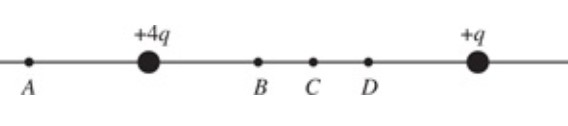
\includegraphics[width=0.55\linewidth]{../figs/PH11-FinalSem2-01-1}
\end{center}
\begin{mcq}(4)
	\item A.
	\item B.
	\item C.
	\item D.
\end{mcq}
\hideall{
\textbf{Đáp án D.}\\
Vì hai điện tích cùng dấu nên vị trí có điện trường tổng hợp bằng 0 phải nằm giữa hai điện tích:
$$\dfrac{k\cdot4q}{r^2_1}=\dfrac{kq}{r^2_2}\Rightarrow r_1=2r_2.$$
}

\item Hai bản kim loại phẳng, tích điện trái dấu, hiệu điện thế giữa hai bản là $\Delta V$. Một electron với khối lượng $m$ và điện tích $e$ ban đầu nằm sát bản tích điện âm. Electron được gia tốc trong vùng không gian giữa hai bản và đạt tốc độ $v$. Nếu hiệu điện thế giữa hai bản được tăng gấp đôi thì electron sẽ đạt được tốc độ bao nhiêu?
\begin{mcq}(4)
	\item $\dfrac{v}{2}$.
	\item $v$.
	\item $\sqrt{2}v$.
	\item $2v$.
\end{mcq}
\hideall{
\textbf{Đáp án C.}\\
Áp dụng định lý động năng:
$$\dfrac{1}{2}mv^2-0=\left|e\right|\Delta V\Rightarrow v=\sqrt{\dfrac{2\left|e\right|U}{m}}.$$
Khi tăng hiệu điện thế giữa hai bản lên 2 lần thì tốc độ của electron tăng $\sqrt{2}$ lần.
}
\textbf{\textit{Dữ kiện dùng chung cho câu 14 - 15}}\\
Các mạch điện dưới dây chứa các điện trở $R$ giống nhau, nguồn điện lý tưởng có suất điện động $V$.
\begin{center}
	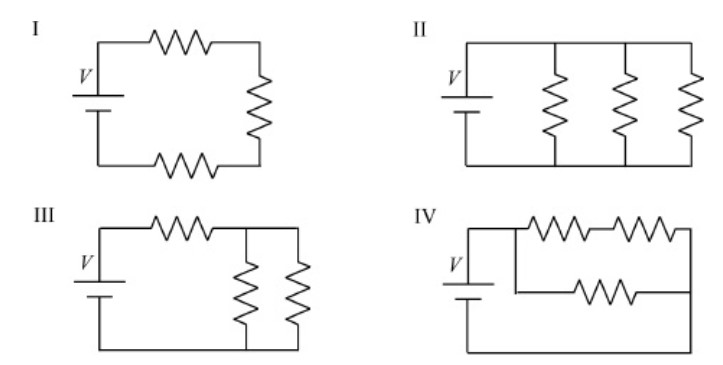
\includegraphics[width=0.6\linewidth]{../figs/PH11-FinalSem2-01-3}
\end{center}
\item Mạch nào sẽ tiêu thụ điện nhiều nhất?
\begin{mcq}(4)
	\item Mạch I.
	\item Mạch II.
	\item Mạch III.
	\item Mạch IV.
\end{mcq}
\hideall{
\textbf{Đáp án B.}\\
Công suất tiêu thụ điện ở mạch ngoài:
$$\calP=\dfrac{V^2}{R_N}.$$
Vì mạch II có điện trở mạch ngoài bé nhất nên tiêu thụ điện nhiều nhất.
}

\item Trong mạch nào thì điện áp giữa hai đầu mỗi điện trở sẽ giống với điện áp của nguồn?
\begin{mcq}(4)
	\item Mạch IV.
	\item Mạch III.
	\item Mạch II.
	\item Mạch I.
\end{mcq}
\hideall{
\textbf{Đáp án C.}
}

\textbf{\textit{Dữ kiện dùng chung cho câu 16 - 18}}\\
Cho mạch điện có sơ đồ như hình vẽ. Bỏ qua điện trở trong của nguồn và dây nối.
\begin{center}
	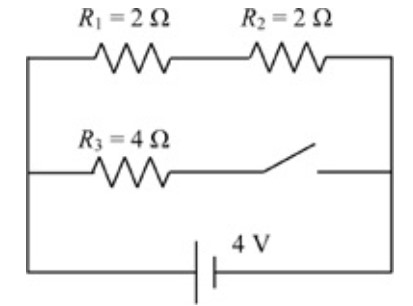
\includegraphics[width=0.35\linewidth]{../figs/PH11-FinalSem2-01-2}
\end{center}
\item Khi công tắc mở, cường độ dòng điện qua mạch là 
\begin{mcq}(4)
	\item $\SI{0.5}{\ampere}$.
	\item $\SI{1.0}{\ampere}$.
	\item $\SI{2.0}{\ampere}$.
	\item $\SI{4.0}{\ampere}$.
\end{mcq}
\hideall{
\textbf{Đáp án B.}\\
Khi công tắc mở, cường độ dòng điện qua mạch:
$$I=\dfrac{\calE}{R_1+R_2}=\SI{1}{\ampere}.$$
}

\item Khi đóng công tắc, điện trở mạch ngoài là
\begin{mcq}(4)
	\item $\xsi{1/2}{\ohm}$.
	\item $\xsi{3/4}{\ohm}$.
	\item $\xsi{4/3}{\ohm}$.
	\item $\SI{2}{\ohm}$.
\end{mcq}
\hideall{
\textbf{Đáp án D.}
}

\item Các điện trở trong mạch thực tế là các bóng đèn. Khi đóng công tắc thì độ sáng của bóng đèn $R_1$ bị ảnh hưởng như thế nào?
\begin{mcq}(2)
	\item Độ sáng giảm đi 1 nửa.
	\item Độ sáng tăng gấp đôi.
	\item Độ sáng giảm 4 lần.
	\item Độ sáng giống nhau.
\end{mcq}
\hideall{
\textbf{Đáp án D.}\\
Cường độ dòng điện qua đèn 1 trước và sau khi đóng công tắc đều bằng $\SI{1}{\ampere}$.
}
\end{enumerate}
\section{Câu trắc nghiệm đúng sai.} 
\textit{Thí sinh trả lời từ câu 1 đến câu 4. Trong mỗi ý \textbf{a)}, \textbf{b)}, \textbf{c)}, \textbf{d)} ở mỗi câu, thí sinh chọn đúng hoặc sai.}
\begin{enumerate}[label=\bfseries Câu \arabic*:]
	\item Trên quảng cáo sản phẩm pin sạc dự phòng của hãng SAMSUNG với tính năng sạc nhanh có công suất sạc $\SI{25}{\watt}$ như hình bên dưới.
	\begin{center}
		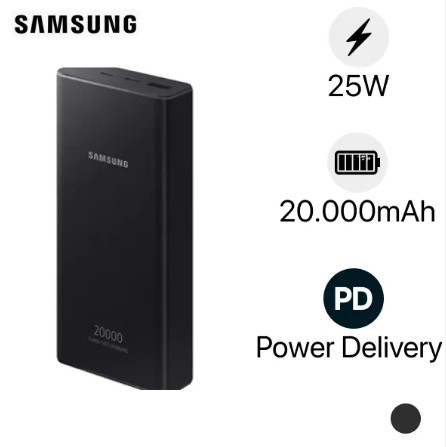
\includegraphics[width=0.4\linewidth]{../figs/PH11-FinalSem2-01-5}
	\end{center}
	\begin{enumerate}[label=\alph*)]
		\item Pin sạc dự phòng tạo ra dòng điện một chiều để nạp điện cho điện thoại.
		\item Thông số $\SI{20000}{\milli\ampere\hour}$ là điện tích cực đại mà pin có thể tích được.
		\item Nếu sử dụng cổng $\SI{2}{\ampere}$ để nạp điện cho điện thoại thì thời lượng sử dụng pin tối đa là $\SI{20}{\hour}$.
		\item Nếu pin được nạp với điện áp đầu vào $\SI{20}{\volt}$ thì cường độ dòng điện đầu vào tối đa là $\SI{1.5}{\ampere}$.
	\end{enumerate}
	\hideall{
		\begin{enumerate}[label=\alph*)]
			\item Đúng.
			\item Đúng.
			\item Sai. Thời lượng sử dụng với cổng nạp $\SI{2}{\ampere}$ là $\SI{10}{\hour}$.
			\item Sai. Cường độ dòng điện đầu vào tối đa $I=\dfrac{\calP}{U}=\SI{1.25}{\ampere}$.
		\end{enumerate}
	}
	
	\item Có hai tụ điện, trên vỏ tụ điện (A) có ghi $\SI{2.5}{\micro\farad}-\SI{300}{\volt}$, tụ điện (B) có ghi $\SI{2.0}{\micro\farad}-\SI{450}{\volt}$.
	\begin{enumerate}[label=\alph*)]
		\item Con số $\SI{2.5}{\micro\farad}$ cho biết điện dung của tụ điện (A) là $\SI{2.5}{\micro\farad}$.
		\item Tụ (A) không thể hoạt động dưới điện áp $\SI{220}{\volt}$.
		\item Khi hai tụ điện được đặt dưới cùng điện áp (cả hai tụ đều không bị đánh thủng), tụ điện A có khả năng tích điện tốt hơn.
		\item Khi tích điện với điện áp tối đa, tụ điện A tích được điện tích lớn hơn.
	\end{enumerate}
\hideall{
\begin{enumerate}[label=\alph*)]
	\item Đúng. Con số $\SI{2.5}{\micro\farad}$ cho biết điện dung của tụ điện (A) là $\SI{2.5}{\micro\farad}$.
	\item Sai. Điện áp tối đa có thể đặt vào tụ (A) là $\SI{300}{\volt}$. Do đó, tụ (A) có thể hoạt động dưới điện áp $\SI{220}{\volt}$.
	\item Đúng. Điện dung tụ (A) lớn hơn điện dung tụ (B) nên tụ (A) tích điện tốt hơn tụ (B) khi đặt cùng điện áp.
	\item Sai. $Q_\text{A max}=\SI{750}{\micro\coulomb}$, $Q_\text{B max}=\SI{900}{\micro\coulomb}$ nên $Q_\text{B max}>Q_\text{A max}$.
\end{enumerate}
}

\item Dẫn một đường dây điện đôi từ mạng điện chung đến một nhà cách đó $\SI{20}{\meter}$. Biết mỗi sợi dây đơn có một lõi đồng với tiết diện bằng $\SI{0.5}{\milli\meter^2}$, điện trở suất của đồng $\SI{1.8E-8}{\ohm\meter}$. Hiệu điện thế ở cuối đường dây là $\SI{220}{\volt}$. Trong nhà sử dụng các đèn dây tóc với tổng công suất là $\SI{300}{\watt}$, trung bình 5 giờ mỗi ngày.
\begin{enumerate}[label=\alph*)]
	\item Dòng điện trong nhà sử dụng có cường độ là $\SI{2}{\ampere}$.
	\item Nếu điện thế định mức của các đèn là $\SI{220}{\volt}$ thì các đèn cần được mắc nối tiếp với nhau để sáng bình thường.
	\item Điện trở dây dẫn là $\SI{1.44}{\ohm}$.
	\item Điện năng đèn tiêu thụ trong 1 tháng (30 ngày) là $\SI{237.6}{\kilo\watt}$.
\end{enumerate}
\hideall{
\begin{enumerate}[label=\alph*)]
	\item Sai. Cường độ dòng điện trong nhà là $I=\dfrac{\calP}{U}=\dfrac{\SI{330}{\watt}}{\SI{220}{\volt}}=\SI{1.5}{\ampere}.$
	\item Sai. Nếu điện thế định mức của các đèn là $\SI{220}{\volt}$ thì các đèn cần được mắc song song với nhau để sáng bình thường.
	\item Đúng. Điện trở dây dẫn:
	$$R=\rho \dfrac{\ell}{S}=\left(\SI{1.8E-8}{\ohm\meter}\right)\cdot\dfrac{\left(\SI{40}{\meter}\right)}{\SI{0.5E-6}{\meter^2}}=\SI{1.44}{\ohm}.$$
	\item Sai. Điện năng các đèn tiêu thụ trong 1 tháng là:
	$$W=\calP t=\left(\SI{0.33}{\kilo\watt
	}\right)\cdot\left(30\cdot\SI{24}{\hour}\right)=\SI{237.6}{\kilo\watt\hour}.$$
\end{enumerate}
}

\item Có hai bóng đèn  $\text{Đ}_1: \SI{120}{\volt}-\SI{60}{\watt}$ và $\text{Đ}_2: \SI{120}{\volt}-\SI{45}{\watt}$. Mắc hai bóng đèn vào đoạn mạch có điện áp $U=\SI{240}{\volt}$ như sơ đồ bên dưới.
\begin{center}
	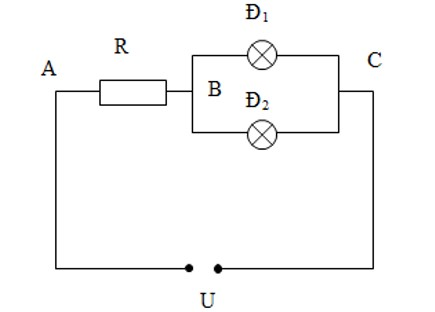
\includegraphics[width=0.4\linewidth]{../figs/PH11-FinalSem2-01-4}
\end{center}
\begin{enumerate}[label=\alph*)]
	\item Điện trở hai đèn có giá trị lần lượt là $R_1=\SI{30}{\ohm}$ và $R_2=\SI{16.875}{\ohm}$.
	\item Hiệu điện thế giữa hai đầu điện trở $R$ khi hai đèn sáng bình thường là $\SI{100}{\volt}$.
	\item Cường độ dòng điện qua đèn 2 luôn nhỏ hơn cường độ dòng điện qua đèn 1.
	\item Để hai đèn sáng bình thường thì điện trở $R$ có giá trị là $\SI{137.14}{\ohm}$.
\end{enumerate}
\hideall{
\begin{enumerate}[label=\alph*)]
	\item Sai. Điện trở mỗi đèn là $R_1=\SI{240}{\ohm}$ và $R_2=\SI{320}{\ohm}$.
	\item Sai. Khi hai đèn sáng bình thường thì hiệu điện thế giữa hai đầu điện trở $R$ là $U_R=U-U_\text{đ}=\SI{120}{\volt}$.
	\item Đúng. Vì hai đèn mắc song song nên $U_\text{đ 1}=U_\text{đ 2}
$ mà $R_2>R_1\Rightarrow I_2<I_1$.
\item Đúng. Hai đèn sáng bình thường thì cường độ dòng điện mạch chính $I=I_1+I_2=\dfrac{\calP_1}{U_1}+\dfrac{\calP_2}{U_2}=\SI{0.875}{\ampere}$. Khi đó:
$$R=\dfrac{U_R}{I}\approx\SI{137.14}{\ohm}.$$


\end{enumerate}
}
\end{enumerate}
\section{Câu trắc nghiệm trả lời ngắn.} \textit{Thí sinh trả lời từ câu 1 đến câu 6.}
\begin{enumerate}[label=\bfseries Câu \arabic*:]
	\item Một pin có suất điện động $\calE=\SI{15}{\volt}$. Công của pin này sinh ra khi có một lượng điện tích $q=\SI{80}{\coulomb}$ dịch chuyển ở bên trong và giữa hai cực của pin là bao nhiêu joule?
	\hideall{
$$A=q\calE=\left(\SI{80}{\coulomb}\right)\cdot\left(\SI{15}{\volt}\right)=\SI{1200}{\joule}.$$	
}

\item Người ta cần quấn biến trở $\SI{100}{\ohm}$ bằng dây nicrom có đường kính tiết diện $\SI{0.4}{\milli\meter}$. Điện trở suất của nicrom là $\rho=\SI{110E-8}{\ohm\meter}$. Chiều dài đoạn dây phải dùng là bao nhiêu mét \textit{(kết quả làm tròn đến 2 chữ số thập phân)}?
\hideall{
$$R=\rho\dfrac{\ell}{S}$$
$$\Rightarrow \ell=\dfrac{R\pi d^2}{4\rho}=\SI{11.42}{\meter}.$$
}

\item Cho mạch điện có sơ đồ như hình vẽ. Nguồn điện có suất điện động $\SI{15}{\volt}$ và điện trở trong $\SI{1}{\ohm}$. Điện trở mạch ngoài có giá trị lần lượt là $R_1=\SI{15}{\ohm}$, $R_2=\SI{5}{\ohm}$, $R_3=\SI{4}{\ohm}$. Cường độ dòng điện qua nguồn là bao nhiêu \textit{(tính theo đơn vị $\si{\ampere}$, lấy 2 chữ số thập phân)}?
\begin{center}
	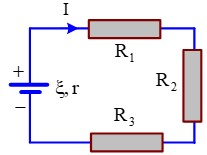
\includegraphics[width=0.25\linewidth]{../figs/PH11-FinalSem2-01-7}
\end{center}
\hideall{
Cường độ dòng điện qua nguồn:
$$I=\dfrac{\calE}{r+R_1+R_2+R_3}=\SI{0.6}{\ampere}.$$
}

	\item Biết rằng khi điện trở mạch ngoài của một nguồn điện tăng từ $R_1=\SI{3}{\ohm}$ đến $R_2=\SI{10.5}{\ohm}$ thì hiệu điện thế giữa hai cực của nguồn tăng gấp hai lần. Điện trở trong của nguồn điện bằng bao nhiêu \textit{(tính theo đơn vị $\si{\ohm}$)}?
	\hideall{
$$U_2=2U_1\Leftrightarrow \dfrac{\calE R_2}{R_2+r}=2\cdot\dfrac{\calE R_1}{R_1+r}\Rightarrow r=\SI{7}{\ohm}.$$	
}

\item Một nguồn điện không đổi có suất điện động $\SI{9}{\volt}$, điện trở trong $\SI{1}{\ohm}$ được nối với mạch ngoài gồm hai điện trở giống nhau mắc nối tiếp thì cường độ dòng điện qua nguồn là $\SI{1}{\ampere}$. Nếu hai điện trở ở mạch ngoài mắc song song thì cường độ dòng điện qua nguồn là bao nhiêu \textit{(tính theo đơn vị $\si{\ampere}$)}?
\hideall{
\begin{itemize}
	\item Khi hai điện trở mạch ngoài mắc nối tiếp:
	$$I=\dfrac{\calE}{r+2R}\Rightarrow R=\dfrac{1}{2}\cdot\left(\dfrac{\calE}{I}-r\right)=\SI{4}{\ohm}.$$
	\item Khi hai điện trở mạch ngoài mắc song song:
	$$I'=\dfrac{\calE}{r+0,5R}=\SI{3}{\ampere}.$$
\end{itemize}
}



\item Cho mạch điện có sơ đồ như hình vẽ, trong đó nguồn điện có suất điện động $\SI{9}{\volt}$, điện trở trong $r=\SI{0.5}{\ohm}$. Các điện trở có giá trị lần lượt là $R_1=\SI{4.5}{\ohm}$; $R_2=\SI{6}{\ohm}$; $R$ là biến trở. Điện trở $R$ phải có giá trị bao nhiêu \textit{(tính theo đơn vị $\si{\ohm}$)} để công suất tiêu thụ điện trên điện trở $R_1$ là lớn nhất?
\begin{center}
	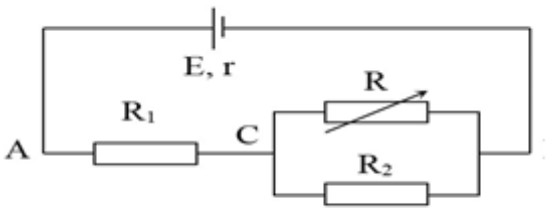
\includegraphics[width=0.4\linewidth]{../figs/PH11-FinalSem2-01-6}
\end{center}
\hideall{
$$\calP_1=\dfrac{\calE^2 R_1}{\left(r+R_1+R_\text{BC}\right)^2}\le \dfrac{\calE^2 R_1}{\left(r+R_1\right)^2}.$$
Như vậy, $\calP_\text{1 max}\Leftrightarrow R=\SI{0}{\ohm}.$
}

\end{enumerate}
\begin{center}
	\textbf{--- HẾT ---}
\end{center}